\chapter{Theoretical Foundations}
\label{ch:foundations}

\section{\glsentrylong{bpmn}}
\label{sec:bpmn}

\gls{bpm} is the act of representing a business process \citep{Silver2011}. Modeling requires a standardized notation that allows for consistent model representation and this is achieved in the \gls{bpm} field by the \gls{bpmn} which is a graphical representation of a semantic process \citep{Silver2011}. \gls{bpmn} is thus to be understood as a language used to draw diagrams \ie a diagramming language \citep{Silver2011}. Its most favorable point is that it is a standard maintained by the \gls{omg} and that it is widely adopted worldwide \citep{Silver2011}. \citet{Silver2011} outlines two fundamental principles that \gls{bpmn} should adhere to:

\begin{enumerate}[label=\textbf{P. \Roman*},ref=Principle \Roman*]
 	\item ``A given \gls{bpmn} diagram should have one and only one interpretation. The process logic should be completely and unambiguously described by the diagram alone.'' \citep[p. v]{Silver2011}. \label{bpmn:p1}
 	\item ``A given \gls{bpmn} diagram should have one and only one \gls{xml} serialization. Otherwise model interchange between tools cannot be achieved.'' \citep[p. v]{Silver2011}. \label{bpmn:p2}
\end{enumerate} 

\ref{bpmn:p1} is more modelers-oriented with no necessary implementation knowledge that should be able to fully understand a diagram by looking at it, while \ref{bpmn:p2} applies more to implementers and process interpreters \citep{Silver2011}.

\citet{Silver2011} differentiates between two important concepts:
\begin{enumerate*}
	\item Activities
	\item Processes.
\end{enumerate*}

Activities are to be understood as units of work performed, or as \citet{Silver2011} defines them: discrete actions with well-defined start and end that are performed repeatedly in the course of business, whose instances can be arbitrarily repeated \citep[p. 10]{Silver2011}. More informally one can see each activity instance as a token that is being generated at a starting state and during its lifetime it will follow a path following the process flow. On the other hand, processes are sequence of actions that lead from a start state to and end state \citep[p. 11]{Silver2011}.

Modeling such processes is done by relying as previously mentioned on \gls{bpmn} in which different building blocks are defined \citep{Silver2011}. A traditional model designed following the \gls{bpmn} guidelines can be found in \figref{fig:normal_process}.

\fig[\textwidth]{normal_process}{\glsentryshort{bpmn} process which shows the most important shapes used}{fig:normal_process}

In the following paragraphs the different elements outlined are explained and \figref{fig:bpmn_elements} gives an overview of the graphical representation in \gls{bpmn} of them.

\fig[\textwidth]{bpmn_elements}{\glsentryshort{bpmn} elements}{fig:bpmn_elements}

\subsection{Start Event}

The main purpose of start events is to indicate where a process starts and it is a strict requirement set by \gls{bpmn} that each process must have such one and at most one \citep{Silver2011}. Technically, start events are those process elements that generate tokens that flow through a process which when they reach a user task get worked by the assigned user.

\subsection{User Task}

Activities are defined by \citet{Silver2011} as atomic units of work that are performed in a process. They are the only elements that assign a performer to them \citep{Silver2011}. For the purpose of this thesis, the only type of activities considered is the user task. They get a user assigned which will work the token that has reached this task.

\subsection{Gateway}

Diamond shaped gateways are elements that control the tokens flow inside a process by effectively splitting its path into alternative ones \citep{Silver2011}. There are three main types of gateways:
\begin{enumerate*}
	\item \gls{xor}
	\item Parallel
	\item \gls{or}.
\end{enumerate*}

\gls{xor} gateways define exclusivity among the alternative paths a token can flow through, meaning that only one path can be pursued per instance \citep{Silver2011}. \gls{xor} gateways do not make decisions, they merely test conditions to activate a specific path \citep{Silver2011}. The decision making process is left to tasks \citep{Silver2011}.

Parallel gateways, in contrast to \gls{xor} gateways, unconditionally split and duplicate the flow of a token inside a process \citep{Silver2011}.

Last but not least, \gls{or} gateways are in a way similar to \gls{xor} gateways since they also have conditional flows but each condition is independent \ie more than one can be true and if that is the case, then the paths are split following the parallel gateway logic \citep{Silver2011}. Normally, \gls{or} gateways always have a default path to be followed \citep{Silver2011}.

\subsection{End Event}

End events indicate the end of the path for a token inside the process \citep{Silver2011}. In contrast to start events, it is possible to have multiple end events \citep{Silver2011}. As soon as a token reaches an end event, the corresponding activity instance is completed.

\section{\glsentrylongpl{wfms} Limitations}

Even though \gls{bpmn} advocates for a formal semantic definition, there are formal gaps in more complex semantic constructs which are under-specified that should be accounted for when modeling processes with \gls{bpmn} \citep{Soerensen2005}. \citet{Soerensen2005} mentions the most critical specification areas lacking formal semantics:
\begin{enumerate*}
	\item \gls{or} gateways with arbitrary number of cycles
	\item Cyclic processes in general
	\item Processes presenting deadlocks that might not ensure termination of progress.
\end{enumerate*}

Both \figref{fig:repeat_loops} and \figref{fig:while_loops} show the representation of two different types of cyclic diagrams that can cause problems, as outlined by \citet{Soerensen2005}.

\begin{figure}[!ht]
	\centering
	\begin{minipage}[b]{0.45\textwidth}
		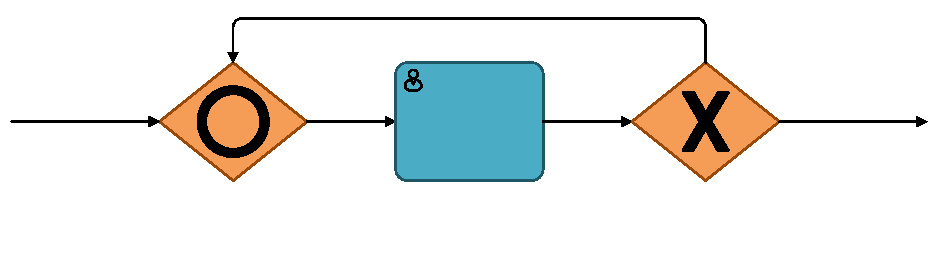
\includegraphics[width=\textwidth]{img/repeat_loops}
		\caption{Cyclic diagram with repeat loop (own plot based on \citet[p. 12]{Soerensen2005})}
		\label{fig:repeat_loops}
	\end{minipage}
	\hfill
	\begin{minipage}[b]{0.45\textwidth}
		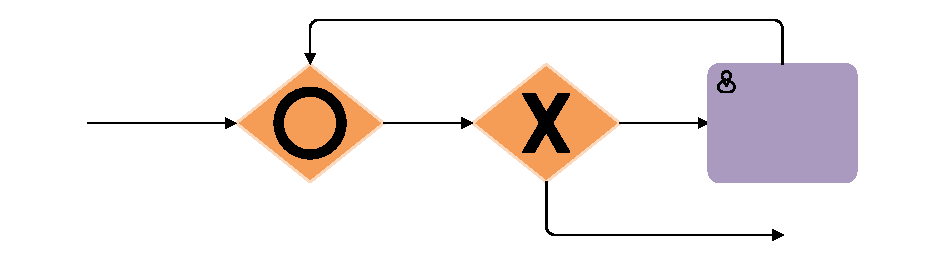
\includegraphics[width=\textwidth]{img/while_loops}
		\caption{Cyclic diagram with while loop (own plot based on \citet[p. 12]{Soerensen2005})}
		\label{fig:while_loops}
	\end{minipage}
\end{figure}

As it is out of scope for this thesis to reiterate over \citet{Soerensen2005}'s work on cyclic processes, we only model and subsequently simulate acyclic processes.

In a real world adoption of \glspl{wfms} bottlenecks can be encountered on each stage along a process. In the simulation environment proposed in this thesis, however, the focus is put only on user tasks and all other process elements are considered to be executed instantly.

\section{Role Resolution}
\label{sec:role_resolution_theory}

As mentioned in \secref{sec:bpmn}, user task elements get users assigned which then work tokens that reach this specific task. The concept of assigning a user to a token (or task) is referred to in the literature as role resolution \citep{Zeng2005,Cheng2000}. When referring to \figref{fig:normal_process}, we see that tokens are being generated by the left most start event and immediately reach a user task. Let us moreover assume that we have a pool of different users that all qualify to process the process token at this specific user task, however the all exhibit different skills level and at the time of arrival they are also variously occupied. The act of choosing the best user under consideration of different process environment factors is that of role resolution \citep{Zeng2005}. Formally, applying role resolution is done by following predefined policies which govern how users are being effectively assigned to work tokens \citep{Zeng2005}. As already mentioned, this thesis focuses on extending the foundations laid by \citet{Zeng2005} in which they define five different types of policies for effective role resolution.

In order to effectively test different polices governing role resolution in \glspl{wfms}, in this thesis a simulation environment has been prepared. By means of simulating processes with different policies acting as supervisors, different metrics can be evaluated to assess one policy's efficiency. Role resolution in this simulation environment happens on a per user task basis \ie when a token reaches a user task, a policy follows its internal definitions on how to optimally assign available users to this token. A simulation environment has been implemented since on one hand it allows to generate the required amount of data relatively fast (which in a real world situation not only could prove to be hard to obtain, but extremely costly as well) and on the other hand, it allows to equally test all role resolution policies by ensuring that they all undergo the exact same processes.